\section{System calls e forking}
Il kernel e' il nucleo del sistema operativo, gestisce le funzioni di controllo fondamentali del computer. 

Ad ogni boot il kernel verifica lo stato delle periferiche, monta la prima partizione in read-only e lancia il primo programma (/sbin/init). Le altre operazioni vengono gestite da programmi eseguiti dal kernel. Permette ai programmi di accedere alle periferiche.

L'interazione tra programmi e il resto del sistema e' mascherata, ogni programma vede se stesso come unico possessore della CPU, quindi non puo' disturbare altri programmi.

\subsection{Privilegi}


\begin{itemize}
  \item User space: ambiente in cui vengono eseguiti i programmi (Ring 3)
  \item Kernel space: ambiente in cui viene eseguito il kernel (Ring 0)
  \item Ring 1, 2 sono dedicati ai driver (non usati da Linux e Windows)
\end{itemize}

\subsection{System calls}
Eseguite nel Kernel Space, sono le interfacce con cui i programmi richiedono servizi dal Kernel, restituiscono i risultati nello user space.

Restituiscono '-1' in caso di errore e settano la var. glob. \textbf{errno} seguendo lo standard POSIX.

\subsubsection{Librerie di sistema}
Una libreria è un insieme di funzioni o strutture dati predefinite e predisposte per essere collegate ad un programma software attraverso un opportuno collegamento. Il collegamento può essere statico o dinamico, nel caso delle librerie di sistema il collegamento è dinamico (dynamic linking).

Il programma shell \textbf{ldd} \textit{(acronimo di List Dynamic Dependencies)} esegue il programma che gli viene dato come argomento e non dovrebbe essere utilizzato con binari non fidati. Visualizza le librerie che il programma carica. ldd e' alias di \texttt{objdump -p /path/program | grep NEEDED}

\begin{itemize}
  \item \textbf{ld-linux.so} trova e carica le librerie condivise richieste dal programma, prepara il programma all'esecuzione e lo esegue
  \item \textbf{libc.so} libreria nota come glibc, contiene le funzioni basilari più comuni
\end{itemize}

\subsubsection{Get time}
Libreria \texttt{time.h}, funzioni time() e ctime().
\begin{itemize}
    \item \texttt{time()} restituisce il tempo dall'Epoch (00:00:00 UTC, January 1, 1970), misurato in secondi. \href{https://www.tutorialspoint.com/c_standard_library/c_function_time.htm}{WIKI}
    
    \paragraph{Esempio 1: time} \hfill\break
    \lstinputlisting[language=C]{Cap1/esempio1_time.c}

    \item \texttt{ctime()} restituisce una stringa rappresentante l'ora locale basata sull'argomento timer. La stringa ritornata ha il formato: Www Mmm dd hh:mm:ss yyyy. \href{https://www.tutorialspoint.com/c_standard_library/c_function_ctime.htm}{WIKI}
    
    \paragraph{Esempio 2: ctime} \hfill\break
    \lstinputlisting[language=C]{Cap1/esempio2_ctime.c}

\end{itemize}

\subsubsection{Working directory}
Libreria \texttt{unistd.h}, libreria che consente l'accesso allo standard POSIX, funzioni chdir() e getcwd().

\begin{itemize}
    \item \texttt{chdir()} change directory - cambia la directory su cui stiamo lavorando
    \item \texttt{getcwd()} get current working directory - stampa la directory in cui siamo
\end{itemize}

    \paragraph{Esempio 3: chdir}
    \lstinputlisting[language=C]{Cap1/esempio3.c}

%arrivato a slide 9 di
% https://didatticaonline.unitn.it/dol/pluginfile.php/1400885/mod_resource/content/2/Labso2021-Lesson_04.pdf
\subsubsection{Operazioni con i file}

\begin{lstlisting}[language=C]
    int open(const char *pathname, int flags, mode_t mode);
    int close(int fd);
    ssize_t read(int fd, void *buf, size_t count);
    ssize_t write(int fd, const void *buf, size_t count);
    off_t lseek(int fd, off_t offset, int whence);

    FILE *fopen(const char *filename, const char *mode);
    int fclose(FILE *stream)    
\end{lstlisting}
    
Si utilizzano le librerie \texttt{unistd.h} \href{https://www.ibm.com/docs/en/aix/7.2?topic=files-fcntlh-file}{IMB} \href{https://pubs.opengroup.org/onlinepubs/009604499/basedefs/fcntl.h.html}{IEEE} e \texttt{unistd.h}
\paragraph{Duplicazione dei file descriptors:}
Un file descriptor è un \textbf{handle opaco} utilizzato nell'interfaccia tra lo spazio utente e il kernel per \textbf{identificare le risorse di file} / socket. Pertanto, quando si utilizza open() o socket() (chiamate di sistema per interfacciarsi al kernel), viene fornito un descrittore di file, che è un \textbf{numero intero} (sarebbe un indice nella struttura dei processi, ma non ci interessa). Pertanto, se vuoi interfacciarti direttamente con il kernel  usando le chiamate di sistema a read(), write(), close() ecc. l'handle che usi è un file descriptor.

Ogni qualvolta un nuovo file viene aperto da un programma viene creata un'entry nella file table del kernel. Queste \textbf{entry sono indirizzabili da un processo tramite il file descriptor (un numero intero)}.
\\
C'è uno strato di \textbf{astrazione} sovrapposto alle chiamate di sistema, che è l'interfaccia \texttt{stdio}. Ciò fornisce più funzionalità / caratteristiche rispetto alle chiamate di sistema di base. Per questa interfaccia, \textbf{l'handle opaco che ottieni è un FILE*,} che viene restituito dalla chiamata fopen(). Ci sono molte funzioni che usano l'interfaccia stdio fprintf(), fscanf(), fclose(), che sono lì per semplificarti la vita. \textbf{In C, stdin, stdout e stderr sono FILE*, che in UNIX corrispondono rispettivamente ai descrittori di file 0, 1 e 2.}
Semplificando con un elenco:
\begin{itemize}
    \item i File Descriptor (FD) sono interi non negativi (0, 1, 2, ... ) associati ai file aperti
    \item 0, 1, 2 sono standard FD che corrispondono agli \texttt{STDIN\_FILENO,STDOUT\_FILENO e STDERR\_FILENO} (definiti in unistd.h) aperti di default quando un programma shell viene eseguito
    \item gli FD di un processo particolare possono essere visti in /proc/$\$$pid/fd (in un sistema Unix based)
\end{itemize}

\begin{figure}[h]
    \centering
    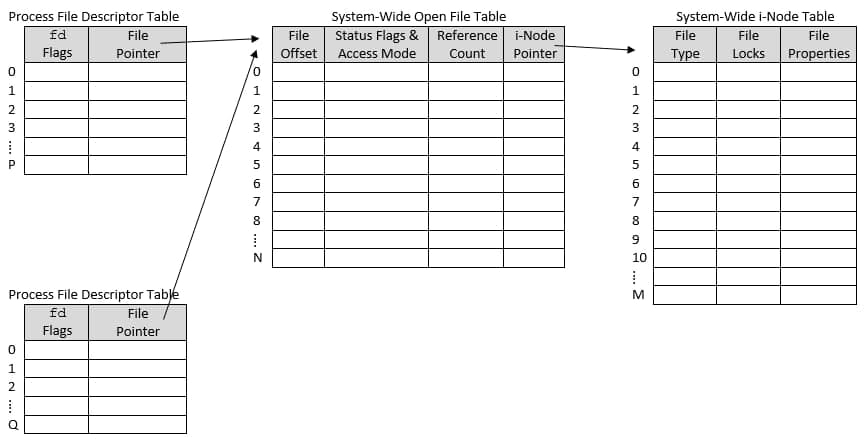
\includegraphics[width=0.85\textwidth]{fds.jpg}
    \caption{Wow such cool}
\end{figure}


\paragraph{Operazioni sugli FD: dup(), dup2()}
Libreria \texttt{unistd.h}\\
    \texttt{    int dup(int oldfd)}\\
    \texttt{    int dup2(int oldfd, int newfd)}\\ \\
Le funzioni dup() e dup2() creano una copia del file descriptor oldfd.
La funzione dup() attribuisce al nuovo file descriptor, il piu' piccolo intero non usato.
La funzione dup2() crea newfd come copia di oldfd, chiudendo prima newfd se e' necessario.

Il vecchio e nuovo file descriptor possono essere utilizzati interscambiabilmente. Essi condividono locks, puntatiori di file position e flag, ad eccezione del flag close-on-exec.
Per Esempio e' possibile effettuare una lseek() su un file descriptor e ritorvarsi la posizione modificata su entrami i file descriptor. 



\paragraph{Esempio 4: dup e dup2}\hfill \break
\lstinputlisting[language=C]{Cap1/esempio4_dup.c}

\paragraph{Esempio: (non ha file C)}
Stai scrivendo un programma shell e vuoi che ridiriga stdin e stdout in un processo figlio. Dovrebbe assomigliare a:
\begin{lstlisting}[language=C]
fdin = open(infile, O_RDONLY);
fdout = open(outfile, O_WRONLY);
// Check for errors, send messages to stdout.
...
int pid = fork();
if(pid == 0) {
    close(STDIN_FILENO);
    dup2(fdin, STDIN_FILENO);

    close(STDOUT_FILENO);
    dup2(fdout, STDOUT_FILENO);
    
    execvp(program, argv);
}
// Parent process cleans up, maybe waits for child.
...
\end{lstlisting}

\subsubsection{Permessi}
Libreria \texttt{sys/stat.h e fcntl.h}\\
%cosa sono i permessi e a cosa servono
%comandi ed esempi
Sebbene ci siano già molte buone funzionalità di sicurezza integrate nei sistemi basati su Linux, può esistere una potenziale vulnerabilità quando viene concesso l'accesso locale, ossia problemi basati sui \textbf{permessi dei file dovuti} da un utente che non assegna i permessi corretti a file e directory.
\paragraph{Proprietà dei file Linux}
Ad ogni file e directory sul tuo sistema Unix / Linux vengono assegnati \textbf{3 tipi di proprietario}:
\begin{itemize}
    \item \textbf{(u) User - Utente è il proprietario del file. } Per impostazione predefinita, la persona che ha creato un file diventa il suo\textbf{ proprietario (owner)}.
    \item \textbf{(g) Group - Gruppo di utenti può contenere più utenti. Tutti gli utenti che appartengono a un gruppo avranno le stesse autorizzazioni del gruppo Linux per accedere al file.} Supponi di avere un progetto in cui un numero di persone richiede l'accesso a un file. Invece di assegnare manualmente le autorizzazioni a ciascun utente, è possibile aggiungere tutti gli utenti a un gruppo e assegnare l'autorizzazione del gruppo al file in modo che solo i membri del gruppo e nessun altro possano leggere o modificare i file.
    \item \textbf{(o) Other - Qualsiasi altro utente che abbia accesso a un file.} Questa persona non ha creato il file, né appartiene a un gruppo utenti che potrebbe possedere il file. In pratica, significa tutti gli altri. Pertanto, quando si imposta l'autorizzazione per gli altri, viene anche definita autorizzazioni impostate per il mondo.
\end{itemize}
Come fa Linux a distinguere tra questi tre tipi di utente in modo che un \textit{utente "A" non possa influenzare un file che contiene informazioni / dati vitali di altri utenti "B"}? È come se non volessi che il tuo collega, che lavora sul tuo computer Linux, visualizzi le tue immagini. È qui che si inseriscono le autorizzazioni e definiscono il comportamento dell'utente.
\paragraph{Autorizzazioni}
Ogni file e directory nel tuo sistema UNIX / Linux ha i seguenti \textbf{3 permessi definiti per tutti e 3 i proprietari discussi sopra.}
\begin{itemize}
    \item \textbf{(r) Read - Lettura}: questa autorizzazione ti dà l'\textbf{autorità di aprire e leggere un file}. Il permesso di lettura su una directory ti dà la possibilità di elencarne il contenuto.
    \item \textbf{(w) Write - Scrittura}: l'autorizzazione di scrittura consente di \textbf{modificare il contenuto di un file}. L'autorizzazione di scrittura su una directory ti dà l'autorità per aggiungere, rimuovere e rinominare i file archiviati nella directory. Si consideri uno scenario in cui è necessario l'autorizzazione di scrittura sul file ma non l'autorizzazione di scrittura sulla directory in cui è archiviato il file. Potrai modificare il contenuto del file. Ma non sarai in grado di rinominare, spostare o rimuovere il file dalla directory.
    \item \textbf{(x) Execute - Esegui}: in Windows, un programma eseguibile di solito ha un'estensione ".exe" e che puoi eseguire facilmente. In Unix / Linux, non è possibile eseguire un programma a meno che non sia impostata l'autorizzazione di esecuzione. Se l'\textbf{autorizzazione di esecuzione} non è impostata, potresti comunque essere in grado di vedere / modificare il codice del programma (a condizione che siano impostati i permessi di lettura e scrittura), ma non eseguirlo.
\end{itemize}

\paragraph{Metodo testuale}
Scomodo, leggi la wiki se interessato.
\label{sec:permessi}
\paragraph{Metodo numerico}
L'utilizzo dei numeri è un altro metodo che consente di modificare le autorizzazioni per tutti e tre i proprietari, i gruppi e altri contemporaneamente, nonché i bit setuid, setgid e sticky. Questa struttura di base del codice è questa:

\texttt{$\$$ chmod xxx nome file}

Dove xxx è un numero di 3 cifre dove ogni cifra può essere qualsiasi cifra da 0 a 7. La prima cifra si applica alle autorizzazioni per il proprietario, la seconda cifra si applica alle autorizzazioni per il gruppo e la terza cifra si applica alle autorizzazioni per tutti gli altri.

Esempio:
\texttt{$\$$ chmod 754 filename} |
7 -$>$ Owner | 5 -$>$ Group | 4 -$>$ Others

\begin{table}[ht]
    \centering
    \begin{tabular}{c|c|c}\textbf{}
     \textbf{Number} &\textbf{ Permission Type } & \textbf{Symbol} \\
     \hline
     0 & No Permission & --- \\
    1 &	Execute & --x \\
    2 &	Write &	-w-\\
    3 &	Execute + Write & -wx\\
    4 &	Read & r--\\
    5 &	Read + Execute & r-x\\
    6 &	Read + Write & rw-\\
    7 &	Read + Write + Execute & rwx\\
    
    
\end{tabular}
    \caption{Numeri dei permessi}
    \label{tab:permessi}
\end{table}





\href{https://wiki.archlinux.org/title/File_permissions_and_attributes}{wiki} |
\href{https://www.guru99.com/file-permissions.html}{info permessi} |
\href{https://www.linux.com/training-tutorials/understanding-linux-file-permissions/}{altre info sui permessi}\\\newline
\textbf{chmod(), chown()}
\begin{itemize}
    \item \textbf{chmod()} - change mode - modifica i permessi di file e directory
    \item \textbf{chown()} - change owner - modifica il proprietario e/o il gruppo assegnato di uno o più file e directory
\end{itemize}

\begin{lstlisting}[language=C]
    int chown(const char *pathname, uid_t owner, gid_t group)
    int fchown(int fd, uid_t owner, gid_t group)
    int chmod(const char *pathname, mode_t mode)
    int fchmod(int fd, mode_t mode)
\end{lstlisting}
La differenza tra chown e fchown consiste che il primo modifica i permessi del file dal suo percorso, il secondo dal suo Process Id (fd), allo stesso modo per chmod e fchmod.

\paragraph{Esempio 5: chown e chmod}\hfill \break
\lstinputlisting[language=C]{Cap1/esempio5_chown.c}

La funziona chmod() funziona anche con i permessi numerici! 

\subsubsection{Eseguire programmi - correggere libreria e spiegare - dividere i programmi in 'esempi' e formattare meglio}
Libreria \texttt{unistd.h} -- \href{https://linuxhint.com/exec_linux_system_call_c/}{info utili}
\begin{lstlisting}[language=C]
    int execv(const char *path, char *const argv[])
    int execvp(const char *file, char *const argv[])
    int execvpe(const char *file, char *const argv[],
        char *const envp[])
    int execl(const char *path, const char *arg0,...,argn,NULL)
    int execlp(const char *file, const char *arg0,...,argn,NULL)
    int execle(const char *file, const char *arg0,...,argn, NULL,
        char *const envp[])
    int execve(const char *filename, char *const argv[], 
        char *const envp[])
\end{lstlisting}

\paragraph{Esempio 6: execv() }\hfill \break
\lstinputlisting[language=C]{Cap1/esempio6_execv1.c}
\lstinputlisting[language=C]{Cap1/esempio6_execv2.c}

\paragraph{Esempio 7: execle()} \hfill \break
\lstinputlisting[language=C]{Cap1/esempio7_execle1.c}
\lstinputlisting[language=C]{Cap1/esempio7_execle2.c}

\paragraph{Esempio 8: dup2/exec}\hfill \break
\lstinputlisting[language=C]{Cap1/esempio8_dup2_exec.c}

\paragraph{Esempio 9: chiamare la shell, system()}\hfill \break
Se si accede alle cartelle con system bisogna stare attenti perche' si vedono da root.
\lstinputlisting[language=C]{Cap1/esempio9_system.c}
\lstinputlisting[language=C]{Cap1/esempio9_system_copy.c}


\subsection{Fork}
La chiamata di sistema \textbf{Fork viene utilizzata per creare un nuovo processo, chiamato processo figlio, che viene eseguito contemporaneamente al processo che effettua la chiamata fork()} (processo genitore). Dopo aver creato un nuovo processo figlio, entrambi i processi eseguiranno l'istruzione successiva che segue la chiamata di forking. Un processo figlio utilizza lo stesso PC (Program Counter), gli stessi registri della CPU e gli stessi file utilizzati nel processo genitore.

Non accetta parametri e restituisce un valore intero. I valori restituiti dal fork() sono:
\begin{itemize}

    \item \textbf{Valore negativo}: la creazione di un processo figlio \textbf{non è riuscita}.
    \item \textbf{Zero}: \textbf{restituito al processo figlio appena creato}.
    \item \textbf{Valore positivo}: restituito \textbf{al genitore o al chiamante}. Il valore contiene l'\textbf{ID del processo figlio appena creato}.
\end{itemize}

Se la creazione del figlio ha \textbf{successo entrambi i processi ricevono un valore di ritorno}, ma questo è diverso nei due casi:
\begin{itemize}
    \item Il processo padre riceve come valore il nuovo PID del processo figlio
    \item Il processo figlio riceve come valore 0
\end{itemize} 

\href{https://www.geeksforgeeks.org/fork-system-call/}{LINK ALTRE INFO}

\subsubsection{Identificativi dei processi}
\textbf{Ad ogni processo è associato un identificativo univoco per istante temporale}, sono organizzati gerarchicamente (padre-figlio) e suddivisi in insiemi principali (sessioni) e secondari (gruppi). Anche gli utenti hanno un loro identificativo e ad ogni processo ne sono abbinati due: quello reale e quello effettivo (di esecuzione).
\begin{itemize}
    \item PID - Process ID
    \item PPID - Parent Process ID
    \item SID - Session ID
    \item PGID - Process Group ID
    \item UID/RUID - (Real) User ID
    \item EUID - Effective User ID
\end{itemize}
\paragraph{getpid(), getppid()}\hfill \break\\
\texttt{pid$\_$t getpid() : restituisce il PID del processo attivopid$\_$t}\\ 
\texttt{getppid() : restituisce il PID del processo padre}

\paragraph{Esempio 10: getpid e getppid}\hfill \break
\lstinputlisting[language=C]{Cap1/esempio10_getppid_getpid.c}

\subsubsection{Relazione tra i processi}
I processi padre-figlio:
\begin{itemize}
    \item \textbf{Conoscono reciprocamente il loro PID} (ciascuno conosce il proprio tramite getpid(), il figlio conosce quello del padre con \textbf{getppid()}, il padre conosce quello del figlio come valore di ritorno di fork())
    \item Si possono usare altre syscall per semplici interazioni come \texttt{wait e waitpid }
    \item Eventuali variabili definite prima del fork sono valorizzate allo stesso modo in entrambi: se riferiscono risorse (ad Esempio un “file descriptor” per un file su disco) fanno riferimento esattamente alla stessa risorsa.
\end{itemize} 

\subsubsection{Processi zombie e orfani}
\paragraph{wait(), waitpid()}
Librerie usate: \texttt{sys/types.h> e <sys/wait.h>}\\

La funzione \texttt{wait()} \textbf{sospende il processo corrente finche' un figlio (child) termina} o finche' il processo corrente riceve un segnale di terminazione o un segnale che sia gestito da una funzione.
Quando un \textbf{child termina il processo, senza che il parent abbia atteso la sua terminazione} attraverso la funzione di wait(), allora il child assume lo \textbf{stato di "zombie" } ossia di processo "defunto".
Se il processo corrente \textbf{esegue la funzione di wait(), in presenza di child in stato di zombie, allora la funzione ritorna immediatamente e ciascuna risorsa del child viene liberata.}

La funzione \texttt{waitpid()} \texttt{sospende il processo corrente finche' il figlio (child) corrispobndente al pid passato in argomento termina} o finche' il processo corrente riceve un segnale di terminazione o un segnale che sia gestito da una funzione.
Se il processo corrente \textbf{esegue la funzione di waitpid() e il child identificato dal pid e' in stato di zombie, allora la funzione ritorna immediatamente e ciascuna risorsa del child viene liberata} (\href{https://stackoverflow.com/questions/20688982/zombie-process-vs-orphan-process}{altre info sui processi zombie}).\\

Il valore del pid puo' essere uno dei seguenti:
\begin{itemize}
    \item -n ($<$-1: attende un qualunque figlio il cui “gruppo” è $|$-n$|$) 
    \item -1 (attende un figlio qualunque)
    \item 0 (attende un figlio con lo stesso “gruppo” del padre)
    \item n (n$>$0: attende il figlio il cui pid è esattamente n)
\end{itemize}

Se \textbf{status non e' NULL, le funzioni wait() e waitpid() memorizzano l'informazione dello stato nell'area di memoria puntata da questo argomento}.\\

Comandi utili:
\begin{lstlisting}[language=C]
    wait(st) corrisponde a waitpid(-1, st, 0)
    while(wait(NULL)>0); # attende tutti i figli    
\end{lstlisting}

Sono disponibili alcune \textbf{macro} per la valutazione dello stato status: 
\begin{itemize}
    \item \textbf{WEXITSTATUS(sts)}: restituisce lo stato vero e proprio (ad Esempio il valore usato nella “exit”)
    \item \textbf{WIFCONTINUED(sts)}: true se il figlio ha ricevuto un segnale
    \item \textbf{SIGCONTWIFEXITED(sts)}: true se il figlio è terminato normalmente
    \item \textbf{WIFSIGNALED(sts)}: true se il figlio è terminato a causa di un segnale non gestito
    \item \textbf{WIFSTOPPED(sts)}: true se il figlio è attualmente in stato di “stop”
    \item \textbf{WSTOPSIG(sts)}: numero del segnale che ha causato lo “stop” del figlio
    \item \textbf{WTERMSIG(sts)}: numero del segnale che ha causato la terminazione del figlio
\end{itemize}

\paragraph{Esempio 11: forking multiplo}\hfill \break
\lstinputlisting[language=C]{Cap1/esempio11_forking_multiplo.c}

\paragraph{Esempio 12: fork$\&$wait}\hfill \break
\lstinputlisting[language=C]{Cap1/esempio12_fork_wait.c}

